\documentclass{beamer}
%\usepackage{xspace}
\usepackage{amsmath,amssymb}
\usepackage{graphicx}
%\usepackage{svg}
%\usepackage{pgfpages}
%\pgfpagesuselayout{4 on 1}[a4paper,border shrink=5mm,landscape]
%\usepackage{psfrag}
%\usepackage[usenames,dvipsnames]{xcolor}
\usepackage{braket}
\usepackage{tikz}
\usepackage{tikz-3dplot}
%\usetikzlibrary{tikz-3dplot}
\usetikzlibrary{graphs}
\usetikzlibrary{datavisualization}
\usetikzlibrary{datavisualization.formats.functions}
\usepackage{pgfplotstable}
\usepgfplotslibrary{patchplots}

\setbeamercovered{transparent}

\usetheme{Pittsburgh}
%\usetheme{default}

\setbeamertemplate{sidebar right}{}
\setbeamertemplate{footline}[frame number]
%\usefonttheme{professionalfonts}

%\usepackage{sansmathaccent}
%\usepackage{bm}

%\usepackage{unicode-math}
%%\setmainfont[SlantedFont={Latin Modern Roman Slanted},SlantedFeatures={Color=000000},
%%  SmallCapsFont={TeX Gyre Termes},SmallCapsFeatures={Letters=SmallCaps}]{XITS}
%\setmathfont[math-style=ISO,sans-style=upright]{XITS Math}
%\setmathfont[range={\mathcal,\mathbfcal}]{Latin Modern Math}

\usepackage{sfmath}

%\mathversion{sans}

\newcommand{\Tr}{\mathsf{Tr}}

\definecolor{redorange}{rgb}{1.0, .25, .25}
\definecolor{citation}{rgb}{.1, 0.8, .35}
\newcommand\emm[1]{\textcolor{redorange}{{#1}}}
\newcommand\numc[1]{\textcolor{citation}{{\bf #1}}}

%\newcommand\bm[1]{{\mbox{\boldmath $#1$}}}
\newcommand\bm[1]{{\mathbf{#1}}}
%\newcommand\bm[1]{{\bf #1}}
%\newcommand\bm[1]{\ensuremath{\boldsymbol{#1}}}
%\newcommand\bm[1]{{\textbf{\it #1}}}

\title{A single qubit}
\author{Ryuhei Mori}
%\institute{$\vcenter{\hbox{\includegraphics[width=30pt]{ELC_logo}}}$ Postdoctoral Fellow of ELC\\ $\vcenter{\hbox{\includegraphics[width=20pt]{titech_logo}}}$ Tokyo Institute of Technology}
\institute{Tokyo Institute of Technology}
%\date{21, Feb, 2019}



\begin{document}
\begin{frame}[plain]
\maketitle
\end{frame}

%\begin{frame}{Operation in a system}
%We will manipulate quantum state.
%
%\vspace{2em}
%This operation can be represented by a map $T: \text{Set of states} \to \text{Set of states}$.
%
%\vspace{2em}
%\end{frame}

\begin{frame}{A single bit}
Let $u=\begin{bmatrix}1\\1\end{bmatrix}$.
\begin{itemize}
\setlength{\itemsep}{2em}
%\item State: \texttt{0},  \texttt{1} and their probabilistic mixture.
%\item Binary measurement: \texttt{0?}, \texttt{1?} and ther linear combination with coefficients in $[0,1]$.
\item 
%\begin{equation*}
$\text{Set of states} = \left\{\omega\in\mathbb{R}^2 \mid \omega\in C_{\ge 0}, \langle u, \omega\rangle = 1\right\}$.
%\end{equation*}
\item 
%\begin{equation*}
$\text{Set of binary measurements} = \left\{e\in\mathbb{R}^2 \mid e\in C_{\ge 0}, u-e \in C_{\ge 0} \right\}$.
%\end{equation*}
\end{itemize}

\vspace{3em}
\centering
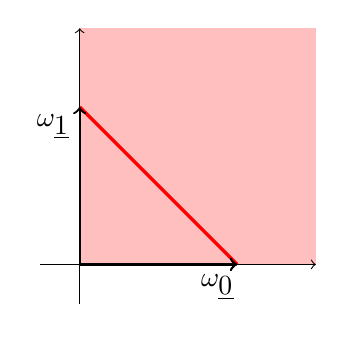
\begin{tikzpicture}
\draw[pink, fill] (0,0) rectangle +(3,3);
\draw[->] (-0.5,0) -- (3,0);
\draw[->] (0,-0.5) -- (0,3);
\draw[very thick, red] (2,0) -- (0,2);
\draw[->, thick] (0,0) -- node[anchor=north, very near end] {$\omega_{\underbar{0}}$} (2,0);
\draw[->, thick] (0,0) -- node[anchor=east, very near end] {$\omega_{\underbar{1}}$} (0,2);
\draw[->, thick] (0,0) -- (2,0);
\end{tikzpicture}
\hfill
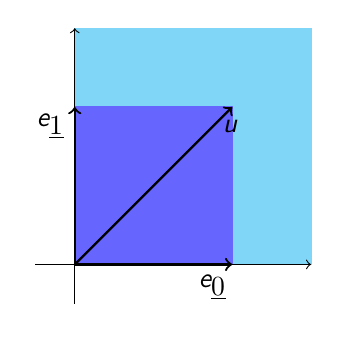
\begin{tikzpicture}
\draw[cyan!50, fill] (0,0) rectangle +(3,3);
\draw[blue!60, fill] (0,0) rectangle +(2,2);
\draw[->] (-0.5,0) -- (3,0);
\draw[->] (0,-0.5) -- (0,3);
%\draw (0,0) -- (2,2);
\draw[->, thick] (0,0) -- node[anchor=north, very near end] {$e_{\underbar{0}}$} (2,0);
\draw[->, thick] (0,0) -- node[anchor=east, very near end] {$e_{\underbar{1}}$} (0,2);
\draw[->, thick] (0,0) -- node[anchor=west, very near end] {$u$} (2,2);
\end{tikzpicture}

%Operation
%\begin{itemize}
%\item Identity: \texttt{0} $\mapsto$ \texttt{0}, \texttt{1} $\mapsto$ \texttt{1}
%\item Bit flip: \texttt{0} $\mapsto$ \texttt{1}, \texttt{1} $\mapsto$ \texttt{0}
%\end{itemize}
\end{frame}

\begin{frame}{A single qubit}
Let $u=\begin{bmatrix}1&0\\0&1\end{bmatrix}$.
\begin{itemize}
\setlength{\itemsep}{2em}
%\item State: A $2\times 2$ Hermitian matrix $\rho$ satisfying $\rho\succeq0$ and $\Tr(\rho)=1$.
%\item Binary measurements: A $2\times 2$ Hermitian matrix $\rho$ satisfying $\rho\succeq0$ and $I-\rho\succeq0$.
\item $\text{Set of states} = \left\{\omega\in V \mid \omega\in C_{\succeq 0}, \langle u,\omega\rangle = 1\right\}$.
\item $\text{Set of binary measurements} = \left\{e\in V \mid e\in C_{\succeq 0}, u-e \in C_{\succeq 0} \right\}$.
\end{itemize}
\begin{tikzpicture}
    \begin{axis}[height= 0.55\vsize, axis lines=center, axis on top, xmin=-1.0, xmax=1.0, ymin=-1.0, ymax=1.0, z buffer = sort, xtick = \empty, ytick=\empty, ztick=\empty ]
    \addplot3[surf, samples= 10, samples y=50, domain= 0:1/sqrt(2), domain y= 0:2*pi, colormap = {pinkpink}{color=(pink) color=(pink)}]
      ({x*cos(deg(y))}, {x*sin(deg(y))}, {x});
    \addplot3[surf, samples= 10, samples y=50, domain= 0:1/sqrt(2), domain y= 0:2*pi, color = red ]
      ({x*cos(deg(y))}, {x*sin(deg(y))}, {1/sqrt(2)});
    \end{axis}
\end{tikzpicture}
\begin{tikzpicture}
    \begin{axis}[height=0.70\vsize, axis lines=center, axis on top, xmin=-1.0, xmax=1.0, ymin=-1.0, ymax=1.0, z buffer = sort, xtick = \empty, ytick=\empty, ztick=\empty ]
    \addplot3[surf, samples= 40, samples y=50, domain= 0:sqrt(2), domain y= 0:2*pi, mesh/interior colormap = {blueblack}{color=(cyan!50) color=(cyan!50)}, colormap = {blueblack}{color=(blue!60) color=(blue!60)}]
      ({(sqrt(2)/2-abs(sqrt(2)/2-x))*cos(deg(y))}, {(sqrt(2)/2-abs(sqrt(2)/2-x))*sin(deg(y))}, {x});
    \end{axis}
\end{tikzpicture}
\end{frame}

\begin{frame}{A single qubit}
\begin{itemize}
\setlength{\itemsep}{3em}
\item A qubit can be represented by
\begin{equation*}
\rho = \frac12\left(I + r_X X + r_Y Y + r_Z Z\right)
\end{equation*}
for $[r_X\, r_Y\, r_Z]\in\mathbb{R}^3$ satisfying $r_X^2+r_Y^2+r_Z^2\le 1$.
\item A qubit can be represented by a point $[r_X\,r_Y\,r_Z]$ in a three-dimensional sphere of radius 1.
\end{itemize}
\end{frame}

\begin{frame}{The Bloch sphere}
\centering

\tdplotsetmaincoords{70}{120}
\begin{tikzpicture}[tdplot_main_coords, scale=2]

%\shade[ball color = lightgray, opacity = 0.5] (0,0,0) circle (1cm);

\tdplotsetrotatedcoords{20}{80}{0}
\draw[very thick, tdplot_rotated_coords] (0,0,0) circle (1);
%\begin{scope}[canvas is zx plane at y=0]
\draw[dashed, thick] (0,0,0) circle (1);
%\end{scope}
 
\draw[-stealth] (0,0,0) -- (2.00,0,0) node[below left] {$X$};
\draw[-stealth] (0,0,0) -- (0,1.80,0) node[below right] {$Y$};
\draw[-stealth] (0,0,0) -- (0,0,1.50) node[above] {$Z$};
 
\end{tikzpicture}
\end{frame}

%\begin{frame}{Spectral decomposition of Hermitian matrix}
%\end{frame}

\begin{frame}{Pauli matrices}
\begin{itemize}
\setlength{\itemsep}{3em}
\item 
\begin{equation*}
Z=\begin{bmatrix}1&0\\0&-1\end{bmatrix}=
\begin{bmatrix}1\\0\end{bmatrix}\begin{bmatrix}1&0\end{bmatrix}
-\begin{bmatrix}0\\1\end{bmatrix}\begin{bmatrix}0&1\end{bmatrix}
\end{equation*}
\item 
\begin{equation*}
X=\begin{bmatrix}0&1\\1&0\end{bmatrix}=
\frac12\begin{bmatrix}1\\1\end{bmatrix}\begin{bmatrix}1&1\end{bmatrix}
-\frac12\begin{bmatrix}1\\-1\end{bmatrix}\begin{bmatrix}1&-1\end{bmatrix}
\end{equation*}
\item 
\begin{equation*}
Y=\begin{bmatrix}0&-i\\i&0\end{bmatrix}=
\frac12\begin{bmatrix}1\\i\end{bmatrix}\begin{bmatrix}1&-i\end{bmatrix}
-\frac12\begin{bmatrix}1\\-i\end{bmatrix}\begin{bmatrix}1&i\end{bmatrix}
\end{equation*}
\end{itemize}
\end{frame}

\begin{frame}{Braket notation}
\begin{align*}
\ket{0} &:= \begin{bmatrix}1\\0\end{bmatrix},&
\ket{1} &:= \begin{bmatrix}0\\1\end{bmatrix}
\end{align*}
\begin{align*}
\ket{+} &:= \frac1{\sqrt{2}}\begin{bmatrix}1\\1\end{bmatrix},&
\ket{-} &:= \frac1{\sqrt{2}}\begin{bmatrix}1\\1\end{bmatrix}\\
&=\frac1{\sqrt{2}}(\ket{0}+\ket{1}),&
&=\frac1{\sqrt{2}}(\ket{0}-\ket{1})
\end{align*}
\begin{align*}
\ket{\psi} = \alpha\ket{0}+\beta\ket{1}=\begin{bmatrix}\alpha\\\beta\end{bmatrix}
\end{align*}
for $|\alpha|^2+|\beta|^2=1$.
\begin{align*}
\bra{\psi} = \ket{\psi}^\dagger = \alpha^*\bra{0}+\beta^*\bra{1}=\begin{bmatrix}\alpha^*&\beta^*\end{bmatrix}
\end{align*}
\end{frame}

\begin{frame}{Pauli matrices in braket notation}
\begin{itemize}
\setlength{\itemsep}{3em}
\item 
\begin{equation*}
Z=\begin{bmatrix}1&0\\0&-1\end{bmatrix}=
\ket{0}\bra{0}
-\ket{1}\bra{1}
\end{equation*}
\item 
\begin{equation*}
X=\begin{bmatrix}0&1\\1&0\end{bmatrix}=
\ket{+}\bra{+}
-\ket{-}\bra{-}
\end{equation*}
\item 
\begin{equation*}
Y=\begin{bmatrix}0&-i\\i&0\end{bmatrix}=
\frac12\begin{bmatrix}1\\i\end{bmatrix}\begin{bmatrix}1&-i\end{bmatrix}
-\frac12\begin{bmatrix}1\\-i\end{bmatrix}\begin{bmatrix}1&i\end{bmatrix}
\end{equation*}
\end{itemize}
\end{frame}

\begin{frame}{Special states}
\begin{equation*}
\rho = \frac12\left(I + r_X X + r_Y Y + r_Z Z\right)
\end{equation*}
\centering
\renewcommand{\arraystretch}{1.5}
\begin{tabular}{|c|c|}
\hline
Coordinate & State\\
\hline
$[0,0,0]$ & $\frac12 I$\\
$[1,0,0]$ & $\frac12 (I+X)=\ket{+}\bra{+}$\\
$[-1,0,0]$ & $\frac12 (I-X)=\ket{-}\bra{-}$\\
$[0,0,1]$ & $\frac12 (I+Z)=\ket{0}\bra{0}$\\
$[0,0,-1]$ & $\frac12 (I-Z)=\ket{1}\bra{1}$\\
\hline
\end{tabular}
\end{frame}

\begin{frame}{Special states in the Bloch sphere}
\centering

\tdplotsetmaincoords{70}{120}
\begin{tikzpicture}[tdplot_main_coords, scale=2]

%\shade[ball color = lightgray, opacity = 0.5] (0,0,0) circle (1cm);

\tdplotsetrotatedcoords{20}{80}{0}
\draw[very thick, tdplot_rotated_coords] (0,0,0) circle (1);
%\begin{scope}[canvas is zx plane at y=0]
\draw[dashed, thick] (0,0,0) circle (1);
%\end{scope}
 
\draw[-stealth] (0,0,0) -- (2.00,0,0) node[below left] {$X$};
\draw[-stealth] (0,0,0) -- (0,1.80,0) node[below right] {$Y$};
\draw[-stealth] (0,0,0) -- (0,0,1.50) node[above] {$Z$};

\filldraw (0,0,0) circle (1pt) node[right] {$I/2$};
\filldraw (1,0,0) circle (1pt) node[below] {$\ket{+}\bra{+}$};
\filldraw (-1,0,0) circle (1pt) node[above] {$\ket{-}\bra{-}$};
\filldraw (0,0,1) circle (1pt) node[above] {$\ket{0}\bra{0}$};
\filldraw (0,0,-1) circle (1pt) node[below] {$\ket{1}\bra{1}$};
 
\end{tikzpicture}
\end{frame}


\begin{frame}{Pure states and state vector}
\begin{align*}
& \text{$\rho$ is a \emm{pure state}}\\
& \overset{\text{def}}{\iff} \rho\ne p\rho_1+(1-p)\rho_2\quad \forall p\in[0,1] \text{ and states $\rho_1,\rho_2\ne\rho$}\\
& \iff \text{$\rho$ is at surface of the Bloch sphere}\\
& \iff r_X^2+r_Y^2+r_Z^2=1\\
& \iff \lambda_1\lambda_2=0 \,\wedge\, \lambda_1+\lambda_2=1\\
& \iff \text{$\rho$ is rank-1 Hermitian with $\Tr(\rho)=1$}\\
& \iff \rho = \ket{\psi}\bra{\psi} \text{ for some $\ket{\psi}\in\mathbb{C}^2$ with $\braket{\psi|\psi}=1$}
\end{align*}

\vspace{1.5em}
Pure state can be represented by a \emm{state vector} $\ket{\psi}\in\mathbb{C}^2$ with $\braket{\psi|\psi}=1$.

\vspace{1em}
$\ket{\psi}$ and $\ket{\varphi}:=\mathsf{e}^{i\theta}\ket{\psi}$ represent the same state since $\ket{\psi}\bra{\psi}=\ket{\varphi}\bra{\varphi}$.
\end{frame}

\begin{frame}{Inner product of pure states}
\begin{itemize}
\item $\rho$ is a qubit pure state with a coordinate $[r_X\,r_Y\,r_Z]$.
\item $\sigma$ is a qubit pure state with a coordinate $[-r_X\,-r_Y\,-r_Z]$.
\end{itemize}
\begin{align*}
\Tr(\rho\sigma) =
\Tr(\rho(I-\rho)) =
\Tr(\rho)-\Tr(\rho^2) =1-1=0
\end{align*}

\vspace{2em}
\begin{itemize}
\item $\rho=\ket{\psi}\bra{\psi}$.
\item $\sigma=\ket{\varphi}\bra{\varphi}$.
\end{itemize}
\begin{align*}
\Tr(\rho\sigma) &=
\Tr(\ket{\psi}\bra{\psi}\ket{\varphi}\bra{\varphi}) =
\braket{\psi|\varphi}\Tr(\ket{\psi}\bra{\varphi})\\
 &= \braket{\psi|\varphi}\braket{\varphi|\psi}
 = |\braket{\psi|\varphi}|^2
\end{align*}
\end{frame}

%\begin{frame}{Classical pure states and operations}
%\end{frame}
\begin{frame}{Unitary operation}
Unitary operation
\begin{equation*}
\rho\mapsto U\rho U^\dagger
\end{equation*}

\vspace{2em}
It is easy to see that
\begin{itemize}
\item $\Tr(U\rho U^\dagger)=1$
\item $U\rho U^\dagger\succeq 0$
\end{itemize}

\vspace{3em}
A pure state $\ket{\psi}$ is mapped to a pure state $U\ket{\psi}$.

\vspace{2em}
$U$ and $\mathsf{e}^{i\theta}U$ play the same role.
\end{frame}

\begin{frame}{Examples of unitary operation}
\begin{itemize}
\setlength{\itemsep}{2em}
\item The identity matrix $I$.
\item Pauli matrices $X$, $Y$ and $Z$.
\item Hadamard matrix $H:=\frac1{\sqrt{2}}\begin{bmatrix}1&1\\1&-1\end{bmatrix}$
\end{itemize}
\end{frame}

\begin{frame}{Pauli matrices $X$ on the Bloch sphere}
\begin{equation*}
\rho = \frac12\left(I + r_X X + r_Y Y + r_Z Z\right)
\end{equation*}
\begin{align*}
X\rho X^\dagger &= X\rho X =  \frac12\left(X^2 + r_X X^3 + r_Y XYX + r_Z XZX\right)\\
&=  \frac12\left(I + r_X X - r_Y Y - r_Z Z\right)
\end{align*}
\begin{align*}
[r_X\,r_Y\,r_Z]\overset{X}{\longmapsto} [r_X\,-r_Y\,-r_Z]
\end{align*}
$\pi$-rotation with respect to $X$ axis.

\vspace{1em}
Similarly, $Y$ and $Z$ corresponds to $\pi$-rotation with respect to $Y$ and $Z$ axes, respectively.
\end{frame}

\begin{frame}{Hadamard matrix}
Hadamard matrix $H$ is unitary and Hermitian.
\begin{align*}
H:=\frac1{\sqrt{2}}\begin{bmatrix}1&1\\1&-1\end{bmatrix}
&=\ket{+}\bra{0}+\ket{-}\bra{1}\\
&=\ket{0}\bra{+}+\ket{1}\bra{-}
\end{align*}
\begin{align*}
\ket{0},\,\ket{1} \overset{H}{\longleftrightarrow} \ket{+},\,\ket{-}
\end{align*}
\begin{align*}
HXH &= H(\ket{+}\bra{+}-\ket{-}\bra{-})H\\
&= \ket{0}\bra{0}-\ket{1}\bra{1} = Z
\end{align*}

Similarly, $HZH=X$.
\end{frame}

\begin{frame}{Hadamard matrix on the Bloch sphere}
\begin{equation*}
\rho = \frac12\left(I + r_X X + r_Y Y + r_Z Z\right)
\end{equation*}
\begin{align*}
H\rho H^\dagger &= H\rho H =  \frac12\left(H^2 + r_X HXH + r_Y HYH + r_Z HZH\right)\\
&=  \frac12\left(I + r_X Z - r_Y Y + r_Z X\right)
\end{align*}
\begin{align*}
[r_X\,r_Y\,r_Z]\overset{H}{\longmapsto} [r_Z\,-r_Y\,r_X]
\end{align*}
Hadamard operation can be decomposed to $\pi/2$-rotation with respect to $Y$ axis
\begin{align*}
[r_X\,r_Y\,r_Z]\overset{R_Y(\pi/2)}{\longmapsto} [-r_Z\,r_Y\,r_X]
\end{align*}
and $X$.
\end{frame}

\begin{frame}{Multiplications of Pauli matrices}
For any unitary matrices $U$ and $V$, $UV$ is also unitary matrix.

\vspace{2em}
\begin{itemize}
\setlength{\itemsep}{2em}
\item $XY=iZ$
\item $YZ=iX$
\item $ZX=iY$
\end{itemize}
\end{frame}

\begin{frame}{Rotation matrices}
\begin{equation*}
R_X(\theta) := \cos\frac{\theta}2 I - i \sin\frac{\theta}2 X
\end{equation*}
\begin{equation*}
R_X(\theta)^\dagger = R_X(-\theta)
\end{equation*}
\begin{align*}
R_X(\theta)R_X(\theta)^\dagger &= (\cos\frac{\theta}2 I - i \sin\frac{\theta}2 X)(\cos\frac{\theta}2 I + i \sin\frac{\theta}2 X)\\
&= \cos^2\frac{\theta}2 I + \sin^2\frac{\theta}2 X^2=I
\end{align*}
\begin{align*}
R_X(\theta)X&=X R_X(\theta),&
R_X(\theta)Y&=Y R_X(-\theta),&
R_X(\theta)Z&=Z R_X(-\theta)
\end{align*}
\begin{align*}
R_X(\theta)R_X(\tau)=R_X(\theta+\tau)
\end{align*}
\begin{align*}
[1\, 0\, 0]&\overset{R_X(\theta)}{\longmapsto} [1\,0\,0]\\
[0\, 1\, 0]&\overset{R_X(\theta)}{\longmapsto} [0\,\cos\theta\,\sin\theta]\\
[0\, 0\, 1]&\overset{R_X(\theta)}{\longmapsto} [0\,-\sin\theta\,\cos\theta]
\end{align*}
%\begin{align*}
%R_X(\theta)\rho R_X(\theta)^\dagger &= \frac12\left(I + r_X X + r_Y R_X(\theta)YR_X(\theta)^\dagger + r_Z R_X(\theta)ZR_X(\theta)^\dagger\right)\\
%&= ...
%\end{align*}
\end{frame}

\begin{frame}{Assignments \small[Deadline is the next of next Friday]}
\begin{itemize}
\setlength{\itemsep}{2em}
\item Show that $R_Y(\theta)=\begin{bmatrix}\cos\frac{\theta}2 & -i\sin\frac{\theta}2\\ \sin\frac{\theta}2 & \cos\frac{\theta}2\end{bmatrix}$
and $R_Z(\theta)=\begin{bmatrix}\mathsf{e}^{-i\theta/2}&0\\0&\mathsf{e}^{i\theta/2}\end{bmatrix}$.
\item Show that for any $2\times 2$ unitary matrix, there exist $\alpha,\,\beta,\,\gamma,\,\delta\in\mathbb{R}$ such that
\begin{equation*}
U=\mathsf{e}^{i\alpha}R_Z(\beta)R_Y(\gamma)R_Z(\delta)
\end{equation*}
\item {[Advanced]} For a real unit vector $\hat{n}=[n_X\,n_Y\,n_Z]$, let
\begin{equation*}
R_{\hat{n}}(\theta):=\cos\frac{\theta}2I -i\sin\frac{\theta}2(n_XX+n_YY+n_ZZ).
\end{equation*}
\end{itemize}
Show that for any $2\times 2$ unitary matrix, there exist $\alpha,\,\theta\in\mathbb{R}$ and a real unit 3d vector $\hat{n}$ such that
$U=\mathsf{e}^{i\alpha}R_{\hat{n}}(\theta)$.
\end{frame}

\begin{frame}{General $2\times 2$ unitary matrices}
$\{I,\,X,\,Y,\,Z\}$ is a orthogonal basis of $2\times 2$ complex matrices.
\begin{equation*}
U=\alpha_I I + \alpha_X X + \alpha_Y Y + \alpha_Z Z 
\end{equation*}
for some $\alpha_I,\alpha_X,\alpha_Y,\alpha_Z\in\mathbb{C}$.
\begin{align*}
UU^\dagger&=(|\alpha_I|^2+|\alpha_X|^2+|\alpha_Y|^2+|\alpha_Z^2|)I\\
&+(\alpha_I\alpha_X^*+\alpha_I^*\alpha_X+i(\alpha_Y\alpha_Z^*-\alpha_Z\alpha_Y^*))X\\
&+(\alpha_I\alpha_Y^*+\alpha_I^*\alpha_Y+i(\alpha_Z\alpha_X^*-\alpha_X\alpha_Z^*))Y\\
&+(\alpha_I\alpha_Z^*+\alpha_I^*\alpha_Z+i(\alpha_X\alpha_Y^*-\alpha_Y\alpha_X^*))Z
\end{align*}
\begin{align*}
\mathsf{Re}(\alpha_I\alpha_X^*) &= \mathsf{Im}(\alpha_Y\alpha_Z^*)\\
\mathsf{Re}(\alpha_I\alpha_Y^*) &= \mathsf{Im}(\alpha_Z\alpha_X^*)\\
\mathsf{Re}(\alpha_I\alpha_Z^*) &= \mathsf{Im}(\alpha_X\alpha_Y^*)
\end{align*}
\end{frame}

\begin{frame}{General rotation matrices}
\begin{align*}
|\alpha_I|^2+|\alpha_X|^2+|\alpha_Y|^2+|\alpha_Z^2|=1
\end{align*}
%\begin{align*}
%\mathsf{Re}(\alpha_I\alpha_X^*) &= \mathsf{Im}(\alpha_Y\alpha_Z^*)\\
%\mathsf{Re}(\alpha_I\alpha_Y^*) &= \mathsf{Im}(\alpha_Z\alpha_X^*)\\
%\mathsf{Re}(\alpha_I\alpha_Z^*) &= \mathsf{Im}(\alpha_X\alpha_Y^*)
%\end{align*}
Assume $\alpha_I$ is real.
\begin{align*}
\alpha_I\mathsf{Re}(\alpha_X) &= \mathsf{Im}(\alpha_Y\alpha_Z^*)\\
\alpha_I\mathsf{Re}(\alpha_Y) &= \mathsf{Im}(\alpha_Z\alpha_X^*)\\
\alpha_I\mathsf{Re}(\alpha_Z) &= \mathsf{Im}(\alpha_X\alpha_Y^*)
\end{align*}
With the direct calculation, we obtain $\alpha_I(\mathsf{Re}(\alpha_X)^2+\mathsf{Re}(\alpha_Y)^2+\mathsf{Re}(\alpha_Z)^2)=0$.
\end{frame}



\end{document}
